\documentclass[utf8]{beamer}
\usepackage{CJKutf8}

%If you want to change the theme, just replace "Bergen" by another theme.

\usetheme{Madrid}
\usecolortheme{seahorse}
\usepackage{graphicx}
\usepackage{xcolor,colortbl}
\usepackage{amsmath, amssymb, amsthm}
\usepackage{listings} %引用程式碼
\usepackage{color}
\usepackage[backend=biber]{biblatex}
\bibliography{rfds.bib}
\usepackage{url}
\def\UrlFont{\tt}
\lstset{
        language=R , %設定語言為R,LaTeX支持各種常見的編程語言,包括C、C++、Java、Matlab、[LaTeX]TeX(認為LaTeX是TeX的一種方言)等等
        escapeinside=`` , %設定`....`之內為逃逸部分,這部分內容將按照正常的LaTeX代碼編譯
        breaklines=true , %設定LaTeX對過長的代碼行進行自動換行
        backgroundcolor=\color{lightgray!40!white} , %設定代碼區底色為淺灰色
        frame=none ,  %設定代碼區不加框
        extendedchars=false , %解決代碼跨頁時,章節標題、頁眉頁腳的漢字無法正常顯示的問題
        keywordstyle=\color{black}\bfseries , %設定相應語言中關鍵字突出顯示方式為藍色、加粗,實現語法高亮
        basicstyle=\ttfamily , %設定代碼的基本字體為等寬字體(類似於Courier)
        commentstyle=\ttfamily\color{purple!60!black} , %設定註釋部分字體為等寬字體,用深綠色顯示
        identifierstyle=\color{black},
        stringstyle=\color{black},
        showstringspaces=false% 設定代碼中字符串的空格正常顯示,而不是顯示為特殊字符“ ␣ ”
        }
        
 \setbeamertemplate{rfds item}{}       
\begin{document}

\begin{CJK}{UTF8}{bsmi}

\title[統計書報]{統計書報}
\institute[NYNSU]{\normalsize{R for Data Science
}\\Strings\&Factors}
\author[吳宗諺]{吳宗諺}

\date{\today}

\begin{frame}
\titlepage
\end{frame}

\begin{frame}{Outline}
\tableofcontents
\end{frame}

\section{字串}
\subsection{字串}
\begin{frame}[fragile]
\frametitle{字串是什麼?}
\begin{itemize}
\item 一段文字。
\item 一種資料的儲存格式,在R裡用一對雙引號""將一段文字夾起來。
\item 混亂的格式,未經處理的資料。
\item 字串裡的雙引號需用單引號夾住。
\end{itemize}
\begin{lstlisting}[language=R,identifierstyle=\color{blue},stringstyle=\color{orange},keywordstyle=\color{green!60!black}\bfseries]
string1 <- "This is a string"
string2 <- ' a "quote" inside a string, use single quotes'
string3 <-"howhowhasfriends9527\\("
\end{lstlisting}
\end{frame}


\subsection{正規表示式}
\begin{frame}
\frametitle{正規表示式是什麼?}
\begin{itemize}
\item 描述符合某個語法規則的字串。
\item 描述字串中的組織與結構。
\item 重要的程式設計工具。
\end{itemize}
\begin{table}[ht]
\centering
表格1.正規表示法的範例\\
\resizebox{\textwidth}{!}{
\begin{tabular}{lrlrlrl}
  \hline
說明 & 正規表示法 & 範例  \\
  \hline
 有小數點的實數 & \lstinline{[0-9]+\\\.[0-9]+}&\textrm{9.527}  \\
 身份證字號 &\lstinline{^[A-Z]\\\d\{9\}$}  & \textrm{A123456789}  \\
  Email &\lstinline{[a-zA-Z0-9_]+@[a-zA-Z0-9\\\._]+} & \textrm{a7788948940@gmail.com}  \\
 中文 &\lstinline{[\\u4e00-\\u9fa5]}& unicode中文編碼範圍  \\
   \hline
\end{tabular}
}
\end{table}
\end{frame}


\begin{frame}
\frametitle{常用的正規表示式}
\begin{table}[ht]
\centering
表格2.常用的正規表示式符號\\
\resizebox{\textwidth}{!}{
\begin{tabular}{lrlrlrl}
  \hline
符號 & 說明 & 範例  \\
  \hline
 \lstinline{\\} &將下一個字元標記為原始字元或者特殊字元 & \lstinline{"\\\."},\lstinline{"\\n"} \\
 \lstinline{^}&匹配輸入字串的結束位置&  \lstinline{"^app"}  \\
 \lstinline{$} &匹配輸入字串的結束位置 &  \lstinline{"le$"}  \\
 \lstinline{*}  &匹配前面的子運算式零次或多次& \lstinline{"7*"}  \\
 \lstinline{+}&匹配前面的子運算式一次或多次& \lstinline{"7+"}  \\
 \lstinline{[]} &括號內的任何字元& \lstinline{"[7]"}  \\
 \lstinline{[^]} &不在括號內的任何字元& \lstinline{"[^7]"}  \\
 \hline
\end{tabular}
}
\end{table}
\end{frame}

\begin{frame}[fragile]
\frametitle{一隻貓走過你的鍵盤}
讓我們看看一種驗證\ Email\ 格式的正規表示法:
\begin{lstlisting}[language=R,identifierstyle=\color{blue},stringstyle=\color{orange},keywordstyle=\color{green!60!black}\bfseries]
((([\t ]*\r\n)?[\t ]+)?[-!#-'*+/-9=?A-Z^-~]+(\.[-!#-'*+/-9=?A-Z^-~]+)*(([\t ]*\r\n)?[\t ]+)?|(([\t ]*\r\n)?[\t ]+)?"(((([\t ]*\r\n)?[\t ]+)?([]!#-[^-~]|(\\[\t -~])))+(([\t ]*\r\n)?[\t ]+)?|(([\t ]*\r\n)?[\t ]+)?)"(([\t ]*\r\n)?[\t ]+)?)@((([\t ]*\r\n)?[\t ]+)?[-!#-'*+/-9=?A-Z^-~]+(\.[-!#-'*+/-9=?A-Z^-~]+)*(([\t ]*\r\n)?[\t ]+)?|(([\t ]*\r\n)?[\t ]+)?\[((([\t ]*\r\n)?[\t ]+)?[!-Z^-~])*(([\t ]*\r\n)?[\t ]+)?](([\t ]*\r\n)?[\t ]+)?)
\end{lstlisting}
\end{frame}

\begin{frame}[fragile]
\frametitle{正規表示法的用途}
\begin{itemize}
\item 處理文字格式的資料(.txt, .html, .csv, ...)
\item 規律性,繁瑣的工作,通常一個正規表示法可以取代大量的迴圈與程式運算。\\
    \begin{itemize}
    \item 元素置換
    \item 指令生成
    \item 驗證格式
    \item 拆解字串
    \end{itemize}
\item 另外,正規表示法幾乎在所有程式語言都是通用的。
\end{itemize}
\end{frame}

\section{學以致用}
\subsection{網路爬蟲–選舉前的PTT八卦版}
\begin{frame}[fragile]
\frametitle{網路爬蟲}
如何獲取資料也是統計的一部份\\
抓取一個網頁的資料:
\begin{lstlisting}[language=R,identifierstyle=\color{blue},stringstyle=\color{orange},keywordstyle=\color{green!60!black}\bfseries]
GET(url,set_cookies("over18"="1"))%>%
  content()%>%
  xml_find_all("//div[@id='main-content']")%>%
  xml_text()%>%stri_conv("UTF-8", "UTF-8")
\end{lstlisting}
在這裡,我們已經用了簡單的正規表示法抓取主文章與留言,但我們想要得更多!
\end{frame}

\begin{frame}[fragile]
\frametitle{抓取巢狀網頁的url}
利用正規表示法抓取巢狀網頁的url,進而生成我們想要的url數量!
\begin{lstlisting}[language=R,identifierstyle=\color{blue},stringstyle=\color{orange},keywordstyle=\color{green!60!black}\bfseries]
GET(url,set_cookies("over18"="1"))%>%
  content()%>%
  xml_find_all("//div[@class='title']/a[@href]")%>%
  xml_attr("href")%>%
  paste('https://www.ptt.cc',., sep='')
\end{lstlisting}
我們可以發現,與抓取一個網頁的程式碼只有正規表示法與抓取物件不同,善用正規表示法可以讓你的程式更為簡化與可讀性。
\end{frame}

\begin{frame}[fragile]
\frametitle{擷取網址}
輕鬆的抓取選舉前十天的文章網址,在這裡我們列出第10000至10003篇的url,最後抓取共近兩萬篇文章的url。
\begin{lstlisting}[language=R,identifierstyle=\color{blue},stringstyle=\color{orange},keywordstyle=\color{green!60!black}\bfseries]
> urls[10000:10003]
 [1] "https://www.ptt.cc/bbs/Gossiping/M.1542634801.A.4F7.html"
 [2] "https://www.ptt.cc/bbs/Gossiping/M.1542634814.A.CAB.html"
 [3] "https://www.ptt.cc/bbs/Gossiping/M.1542634820.A.3E7.html"
 [4] "https://www.ptt.cc/bbs/Gossiping/M.1542634838.A.5D8.html"
\end{lstlisting}
再將這些url丟入爬蟲程式抓取文章與其留言。接著就可以進行文字清理。
\end{frame}

\begin{frame}[fragile]
\frametitle{觀察抓取後的資料}
\begin{lstlisting}[language=R,backgroundcolor=\color{lightgray!0!white},identifierstyle=\color{blue},stringstyle=\color{orange},keywordstyle=\color{green!60!black}\bfseries]
[1] "作者vic2211 (`我是vic`)看板Gossiping標題[`FB`] 中原大學設計學院院長陳其澎時間Mon Nov 19 21:40:12 2018\nFB卦點說明:陳院長光速打臉韓導 說韓導肯定是遇到金光黨了\n\nhttps://www.facebook.com/chiepeng/posts/2415337508482774\n\n\n陳其澎\n9 分鐘 ·\n我是中原大學設計學院院長陳其澎,我發誓我從來沒有見過韓國瑜,更沒有帶五個學生去\n看你的摩天輪,你在說什麼?我完全不知道,你肯定碰到金光黨了。\n\n--\n※ 發信站: 批踢踢實業坊(ptt.cc), 來自: 220.141.18.148\n※ 文章網址: https://www.ptt.cc/bbs/Gossiping/M.1542634814.A.CAB.html... <truncated>
\end{lstlisting}
\end{frame}

\begin{frame}[fragile]
\frametitle{文字清理與字詞分割}
我們更進一步地用自訂義的正規表示法來篩選我們所需要的字詞
\begin{lstlisting}[language=R,backgroundcolor=\color{lightgray!0!white},identifierstyle=\color{blue},stringstyle=\color{orange},keywordstyle=\color{green!60!black}\bfseries]
gsub("[^\u4e00-\u9fa5:]+", "", articles)%>%
    gsub("(`作者`)|(`看板`)|(`標題`)|(`發信站`)|(`批踢踢實業坊`)|(`來自`)|(`文章網址`)|(`編輯`)|(`啊`)|(`喔`)|(`啦`)|(`你`)|(`我`)|(`他`)|(`們`)|(`推`)|(`的`)|(`噓`)|(`了`)|(`是`)|(`就`)|(`人`)|(`不`)|(`在`)|(`有`)|(`都`)|(`要`)|(`沒`)|(`還`)|(`也`)|(`說`)|(`會`)|(`嗎`)+","", .)%>%
    gsub("\n|[ \t]+", "",. )%>%
    str_split(., boundary("word"))
\end{lstlisting}
這裡我們使用內建的字詞分割,即可簡單的分類出詞語。
\end{frame}
\begin{frame}[fragile]
\frametitle{減少資料量}
從表格三可以看出雖然用較多的正規表示法有較久的執行時間,但整體資料量減少了約\ $15\%$ 左右。
\begin{table}[ht]
\centering
表格三.使用正規表示式的比較\\
\resizebox{0.7\textwidth}{!}{
\begin{tabular}{lrlrlll}
  \hline
 & 中文篩選 & 加入自訂義  \\
  \hline
 執行時間(秒)&38.58 & 65.60 \\
 資料大小(Mb)& 511.4& 435.4 \\
 \hline
\end{tabular}
}
\end{table}
\end{frame}

\begin{frame}[fragile]
\frametitle{最終資料}
\begin{lstlisting}[language=R,identifierstyle=\color{blue},stringstyle=\color{orange},keywordstyle=\color{green!60!black}\bfseries]
> final_pttword[2018126:2018166,]
 [1] `可`      `自行`    `提`      `出`      `依據`    `哪個`
 [7] `法`      `但`      `基於`    `法律`    `競合`    `只能`
[13] `擇`      `其一`    `進行`    `求償`    `但`      `無論如何`
[19] `最後`    `看`      `事`      `實`      `調查`    `及`
[25] `法院`    `認定`    `民眾`    `再`      `依據`    `具體`
[31] `個案`    `情況`    `選擇`    `解釋`    `一下`    `為何`
[37] `這個`    `爭論`    `行政院`  `認為`     `高雄市`
59015 Levels:
\end{lstlisting}
\end{frame}

\section{因子}
\subsection{因子}
\begin{frame}[fragile]
\frametitle{因子是什麼?}
\begin{itemize}
\item 一種資料型態。
\item 尺度型的類別變數
\end{itemize}
\begin{lstlisting}[language=R,identifierstyle=\color{blue},stringstyle=\color{orange},keywordstyle=\color{green!60!black}\bfseries]
x1 <- c("9","5","2","7")
levels <- c("1","2","3","4","5","6","7","8","9")
y1 <- factor(x1, levels = levels)
> sort(y1)
[1] 2 5 7 9
Levels: 1 2 3 4 5 6 7 8 9
\end{lstlisting}
\end{frame}

\begin{frame}[fragile]
\frametitle{回到字詞資料}
利用因子的特性,查看各類別資料的頻率
\begin{lstlisting}[language=R,identifierstyle=\color{blue},stringstyle=\color{orange},keywordstyle=\color{green!60!black}\bfseries]
# A tibble: 59,015 x 2
   word      n
   <fct> <int>
 1 `柯`    79895
 2 `台灣`  52996
 3 `韓`    50138
 4 `真`    48193
 5 `好`    46303
 6 `這`    46293
 7 `被`    44610
 8 `文`    43924
# ... with 59,005 more rows
\end{lstlisting}
\end{frame}

\begin{frame}[fragile]
\frametitle{因子視覺化}
挑選感興趣的因子並作圖,利用長條圖觀察各候選人的討論熱度。
\begin{lstlisting}[language=R,identifierstyle=\color{blue},stringstyle=\color{orange},keywordstyle=\color{green!60!black}\bfseries]
x1<-c("柯","姚","丁","台灣","韓","陳","國民黨","民進黨")
factor(final_pttword0$word,levels = x1)%>%
na.omit()%>%data.frame(word=.)%>%
ggplot(., aes(word)) +
  geom_bar()
\end{lstlisting}
\end{frame}

\begin{frame}[fragile]
\frametitle{}
柯候選人的討論頻率明顯高於其他候選人!
\begin{figure}
       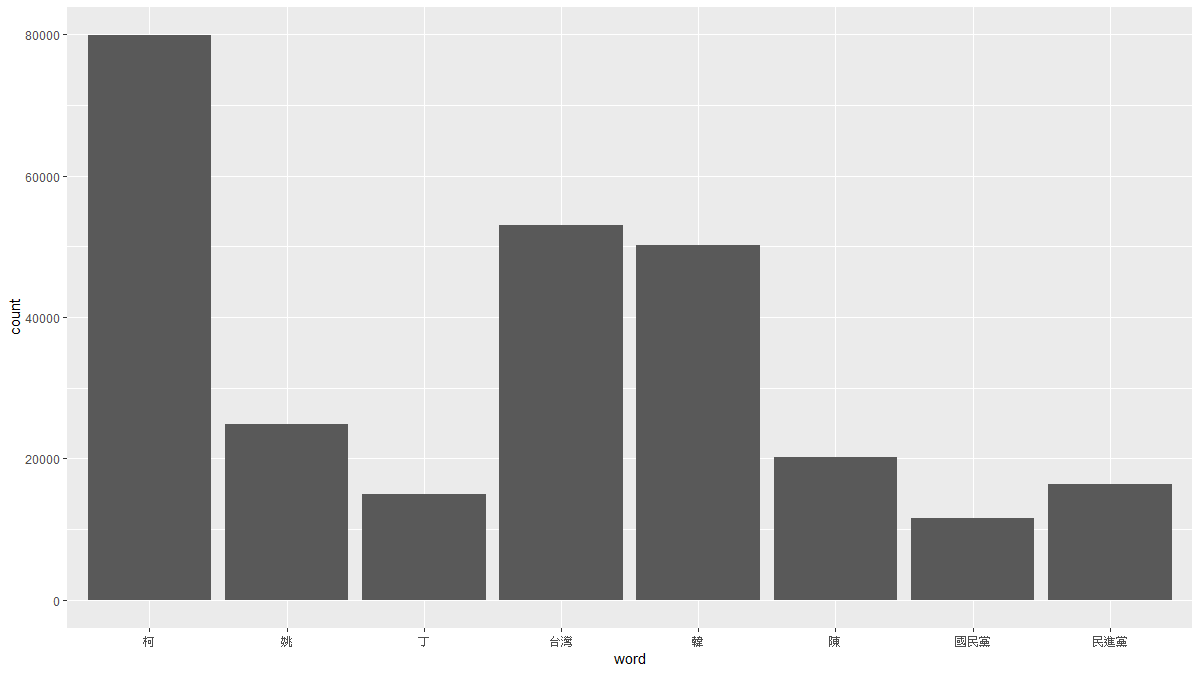
\includegraphics[width=10cm]{plot.png}
      \caption{\label{1}各候選人在八卦版的討論頻率圖}
\end{figure}
\end{frame}

%\section{參考文獻}
%\begin{frame}{參考文獻}
%\printbibliography
%\end{frame}

\begin{frame}
\frametitle{參考文獻}
\href{https://r4ds.had.co.nz/strings.html}
    {\url{Hadley Wickham & Garrett Grolemund(2016).R for Data Science: Import, Tidy, Transform, Visualize, and Model Data,chapter.14.O'Reilly Media}}\\
\href{https://r4ds.had.co.nz/factors.html}
    {\url{Hadley Wickham & Garrett Grolemund(2016).R for Data Science: Import, Tidy, Transform, Visualize, and Model Data,chapter.15.O'Reilly Media}}\\
\end{frame}

\begin{frame}
\begin{center}
This is \alert{The End} of The Presentation\\
And \alert{Thank You} for Your Attention
\end{center}
\end{frame}

\end{CJK}
\end{document} 